\documentclass[xcolor=dvipsname]{beamer} %handout, ignorenonframetext

%\usepackage[ngerman]{babel}
\usepackage[utf8]{inputenc}
\usepackage{amsmath}
\usepackage{graphicx}
\usepackage{subfigure}
\usepackage{multimedia}
\usepackage{wrapfig}
\usepackage{listings}
\usepackage{comment}
\usepackage{framed,color}
\usepackage{listings}


\fboxsep=1pt%padding thickness
\fboxrule=1pt%border thickness
\usepackage{fancybox}

\usepackage{lipsum}
\usepackage{tabularx}
\usepackage{colortbl}
\usepackage{url}


\hypersetup{
	linkcolor=DarkSkyBlue,
	citecolor= DarkSkyBlue,
	filecolor= DarkSkyBlue,
	urlcolor= DarkSkyBlue
}


% COLOR-DEFINITION
%%%%%%%%%%%%%%%%%%%%%%%%
\definecolor{LightButter}{rgb}{0.98,0.91,0.31}
\definecolor{LightOrange}{rgb}{0.98,0.68,0.24}
\definecolor{LightChocolate}{rgb}{0.91,0.72,0.43}
\definecolor{LightChameleon}{rgb}{0.54,0.88,0.20}
\definecolor{LightSkyBlue}{rgb}{0.45,0.62,0.81}
\definecolor{LightPlum}{rgb}{0.68,0.50,0.66}
\definecolor{LightScarletRed}{rgb}{0.93,0.16,0.16}
\definecolor{LightGray}{rgb}{0.80,0.80,0.80}
\definecolor{Butter}{rgb}{0.93,0.86,0.25}
\definecolor{Orange}{rgb}{0.96,0.47,0.00}
\definecolor{Chocolate}{rgb}{0.75,0.49,0.07}
\definecolor{Chameleon}{rgb}{0.45,0.82,0.09}
\definecolor{SkyBlue}{rgb}{0.20,0.39,0.64}
\definecolor{Plum}{rgb}{0.46,0.31,0.48}
\definecolor{ScarletRed}{rgb}{0.80,0.00,0.00}
\definecolor{DarkButter}{rgb}{0.77,0.62,0.00}
\definecolor{DarkOrange}{rgb}{0.80,0.36,0.00}
\definecolor{DarkChocolate}{rgb}{0.56,0.35,0.01}
\definecolor{DarkChameleon}{rgb}{0.30,0.60,0.02}
\definecolor{DarkSkyBlue}{rgb}{0.12,0.29,0.53}
\definecolor{DarkPlum}{rgb}{0.36,0.21,0.40}
\definecolor{DarkScarletRed}{rgb}{0.64,0.00,0.00}



% HPI-THEME
%%%%%%%%%%%%%%%%%%%%%%%%
\RequirePackage{scrlfile}
%\ReplaceFile{beamerthemehpiswa.sty}{theme/beamerthemehpiswa.sty}
%\ReplaceFile{beamercolorthemehpiswa.sty}{theme/beamercolorthemehpiswa.sty}
%\ReplaceFile{beamerfontthemehpiswa.sty}{theme/beamerfontthemehpiswa.sty}
%\ReplaceFile{beamerinnerthemehpiswa.sty}{theme/beamerinnerthemehpiswa.sty}
%\ReplaceFile{beamerouterthemehpiswa.sty}{theme/beamerouterthemehpiswa.sty}
%\ReplaceFile{hpi.png}{theme/hpi.png}
\usetheme{hpiswa}


% BEAMER-Anpassungen
%%%%%%%%%%%%%%%%%%%%%%%%
\setbeamercolor{block title}{bg=DarkOrange}
\setbeamercolor{block body}{bg=Orange!20}
%\setbeamercolor{block title alerted}{bg=red}
\setbeamercolor{block body alerted}{bg=red!20}
%\setbeamercolor{block title example}{bg=green}
\setbeamercolor{block body example}{bg=DarkChameleon!20}
%\usecolortheme[RGB={205,173,0}]{structure}
\usecolortheme[RGB={30,74,135}]{structure}

\usecolortheme{orchid}
%\usefonttheme{professionalfonts}
%\useoutertheme[subsection=false]{smoothbars}
%\useinnertheme{rectangles}
%\setbeamertemplate{blocks}[shadow=true]

\setbeamercovered{transparent}
\setbeamertemplate{navigation symbols}{}%remove navigation symbols



% Eigene Anpassungen
%%%%%%%%%%%%%%%%%%%%

% Explainframes:
\usepackage{ifthen}
\newboolean{isexplainframe}
\setboolean{isexplainframe}{false}
\mode<handout>{
\newenvironment{explainframe}[1]{
\setboolean{isexplainframe}{true}
\addtocounter{framenumber}{-1}
\setbeamertemplate{background}[grid][step=5mm,color=LightGray]
\begin{frame}[fragile,environment=explainframe]{Handout only: #1}%
}{%
\end{frame}%
\setboolean{isexplainframe}{false}
}
\newenvironment{clearexplainframe}[0]{
\setboolean{isexplainframe}{true}
\addtocounter{framenumber}{-1}
\setbeamertemplate{background}[grid][step=5mm,color=LightGray]
\begin{frame}[fragile,environment=clearexplainframe]%
}{%
\end{frame}%
\setboolean{isexplainframe}{false}
}
}
\mode<beamer>{
\excludecomment{explainframe}
\excludecomment{clearexplainframe}
}

\setbeamertemplate{footline}{%
	\leavevmode%
	\hbox{%
		\begin{beamercolorbox}[wd=.45\paperwidth,ht=2.25ex,dp=1ex,center]{author in head/foot}%
			\usebeamerfont{author in head/foot}\insertinstitute
		\end{beamercolorbox}%
		\begin{beamercolorbox}[wd=.2\paperwidth,ht=2.25ex,dp=1ex,center]{title in head/foot}%
			\usebeamerfont{title in head/foot}\insertshorttitle
		\end{beamercolorbox}%
		\begin{beamercolorbox}[wd=.35\paperwidth,ht=2.25ex,dp=1ex,right]{date in head/foot}%
			\usebeamerfont{date in head/foot}\insertshortdate{}\hspace*{2em}
			\insertframenumber{}\ifthenelse{\boolean{isexplainframe}}{E}{} / \inserttotalframenumber\hspace*{2ex}
	\end{beamercolorbox}}%
	\vskip0pt%
}

\definecolor{javared}{rgb}{0.6,0,0} % for strings
\definecolor{javagreen}{rgb}{0.25,0.5,0.35} % comments
\definecolor{javapurple}{rgb}{0.5,0,0.35} % keywords
\definecolor{javadocblue}{rgb}{0.25,0.35,0.75} % javadoc

\lstset{
  language=Ruby,
  basicstyle=\normalsize\ttfamily,
  keywordstyle=\color{javapurple}\bfseries,
  stringstyle=\color{javared},
  commentstyle=\color{javagreen},
  morecomment=[s][\color{javadocblue}]{/**}{*/},
  tabsize=4,
  showspaces=false,
  showstringspaces=false,
  breaklines=true
}


% Gliederung vor jedem Punkt:
\AtBeginSection[]{
\ifthenelse{\equal{\value{section}}{1}}{}{
\ifthenelse{\equal{\value{section}}{6}}{}{
\begin{frame}{Overview}
	\tableofcontents[currentsection, hideothersubsections]
\end{frame}
}
}
}


% Quote-Environment:

\renewenvironment{quote}{%
\begin{exampleblock}{}%
\begin{center}%
\begin{large}%
``}{%
''\end{large}%
\end{center}%
\end{exampleblock}}




% Dokument-Meta-Daten:
%%%%%%%%%%%%%%%%%%%%%%%
\title{Call-target-specific Method Arguments}
\subtitle{ICOOOLPS 2015}
\author{Fabio Niephaus, Matthias Springer, Tim Felgentreff, Tobias Pape, Robert Hirschfeld}
\date{July 6, 2015}
\institute[2012]{Hasso Plattner Institute, Software Architecture Group}



\begin{document}

\begin{frame}[plain]
	\maketitle
\end{frame}
\begin{frame}{Overview}
	\tableofcontents[hideallsubsections]
\end{frame}

\section{Introduction}
\begin{frame}{Introduction}
	\begin{itemize}
		\item Goal: make method calls faster.
		\item How to: prepare arguments for method calls at call site.
		\item Running example: keyword arguments in JRuby --> twice as fast
	\end{itemize}
\end{frame}

\section{Concept}
\begin{frame}[fragile]{Argument Mismatch}
\begin{table}
	\centering
	\textbf{method signature $\not=$ call arguments}
\end{table}

\begin{table}
\begin{minipage}{0.8\textwidth}
\begin{lstlisting}
def method(a: 0, b: 0, c: 0)

end

method(a: 1, b: 2, c: 3)

method(b: 1, a: 2)
method(c: 4)
method()
\end{lstlisting}
\end{minipage} % comment
\begin{minipage}{0.45\textwidth}
%\emph{signature:} \texttt{(a, b, c)} \\ \\ \\ \\
%\emph{arguments:} \texttt{(a, b, c)} \\ \\
%\emph{arguments:} \texttt{(b, a)} \\ 
%\emph{arguments:} \texttt{(c)} \\ 
%\emph{arguments:} \texttt{($\emptyset$)} \\
\end{minipage}
\end{table}
\end{frame}

\begin{frame}{When to Convert Arguments?}
\begin{minipage}{0.49\textwidth}
\begin{table}
\centering
\textbf{convert after invoke:} \newline \newline
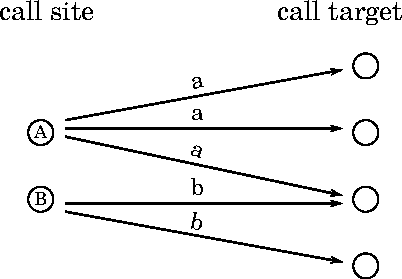
\includegraphics[width=0.8\textwidth]{pic_regular.pdf}
\end{table}
\end{minipage} % comment
\begin{minipage}{0.49\textwidth}
\begin{table}
\centering
\textbf{convert before invoke:} \newline \newline
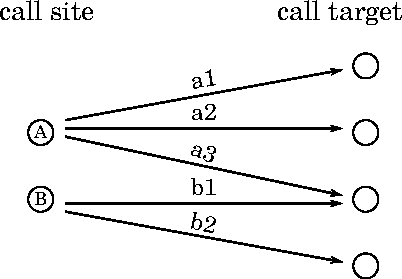
\includegraphics[width=0.8\textwidth]{pic_calltarget.pdf}
\end{table}
\end{minipage}
\end{frame}

\begin{frame}{When to Convert Arguments?}
\begin{minipage}{0.49\textwidth}
\begin{table}
\centering
\textbf{convert after invoke:} \newline \newline
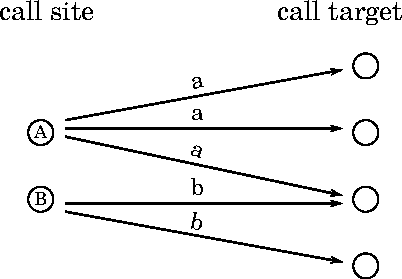
\includegraphics[width=0.8\textwidth]{pic_regular.pdf}
\end{table}
\begin{enumerate}
	\item Convert args to generic repres.
	\item Lookup receiver
	\item Invoke target method
	\item Convert args to specific repres.
\end{enumerate}
\end{minipage} % comment
\begin{minipage}{0.49\textwidth}
\begin{table}
\centering
\textbf{convert before invoke:} \newline \newline
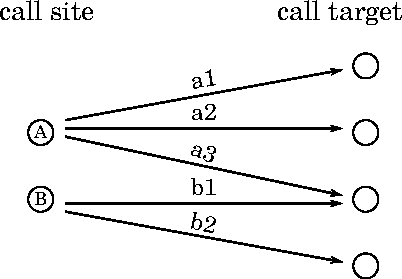
\includegraphics[width=0.8\textwidth]{pic_calltarget.pdf}
\end{table}
\begin{enumerate}
	\item Lookup receiver
	\item Convert args to specific repres.
	\item Invoke target method
\end{enumerate}
\end{minipage}
\end{frame}

\section{Example: Ruby Keyword Arguments}
\begin{frame}[fragile]{Convert After Invocation: Call-site-specific Arguments}
\begin{minipage}{0.25\textwidth}
\centering
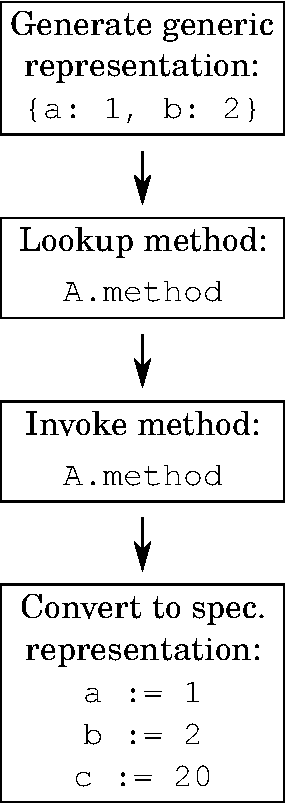
\includegraphics[height=0.8\textheight]{convert_after.pdf}
\end{minipage} % comment
\begin{minipage}{0.7\textwidth}
\begin{lstlisting}
def A.method(b: 10, c: 20, a: 30)
end

obj.method(a: 1, b: 2)
\end{lstlisting}
\end{minipage}
\end{frame}

\begin{frame}[fragile]{Convert Before Invocation: Call-target-specific Arguments}
\begin{minipage}{0.3\textwidth}
\centering
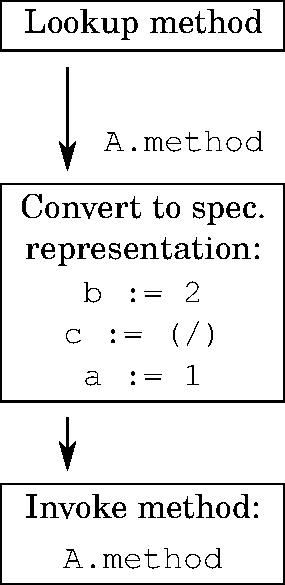
\includegraphics[height=0.6\textheight]{convert_before.pdf}
\end{minipage} % comment
\begin{minipage}{0.65\textwidth}
\begin{lstlisting}
def A.method(b: 10, c: 20, a: 30)
end

obj.method(a: 1, b: 2)
\end{lstlisting}
\end{minipage}
\end{frame}


\begin{frame}[fragile]{Convert Before Invocation: Call-target-specific Arguments}
\begin{minipage}{0.55\textwidth}
\centering
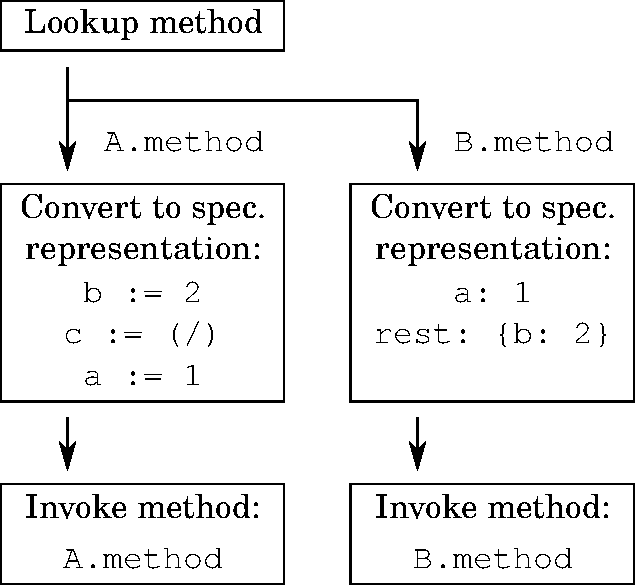
\includegraphics[height=0.6\textheight]{convert_before2.pdf}
\end{minipage} % comment
\begin{minipage}{0.4\textwidth}
\begin{lstlisting}
def A.method(b: 10, c: 20, a: 30)
end

def B.method(a:, **rest)
end

obj.method(a: 1, b: 2)
\end{lstlisting}
\end{minipage}
\end{frame}

\begin{frame}[fragile]{Convert Before Invocation: Call-target-specific Arguments}
\begin{minipage}{0.55\textwidth}
\centering
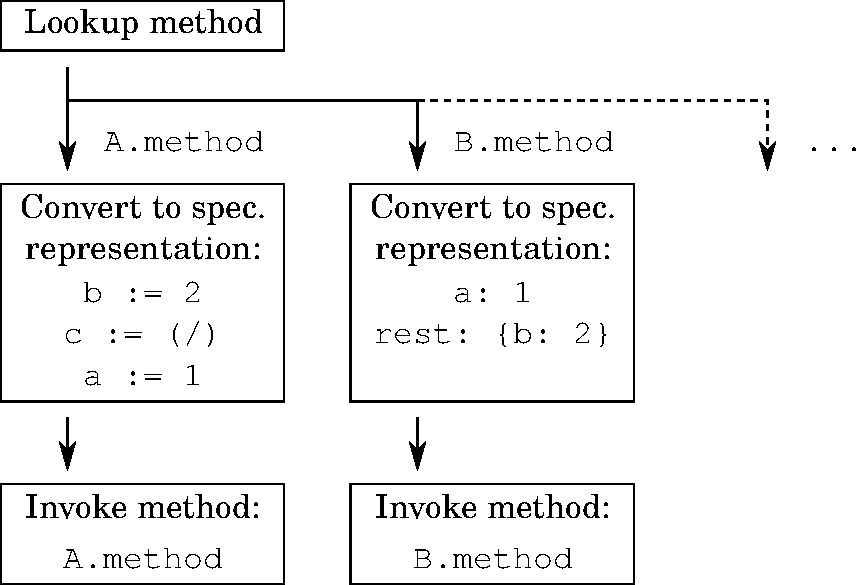
\includegraphics[height=0.6\textheight]{convert_before3.pdf}
\end{minipage} % comment
\begin{minipage}{0.4\textwidth}

\end{minipage}
\end{frame}

\begin{frame}{Call-target-specific Method Arguments}
\begin{itemize}
	\item Code/AST for generating arguments representation depends on call target.
	\item We cache one AST subtree generating the arguments array per PIC entry.
	\item Call-target-specific argument handling is part of the PIC.
\end{itemize}
\end{frame}

\section{Implementation Details}

\section{Benchmarks}
\begin{frame}{Micro-Benchmarks}
	\centering
	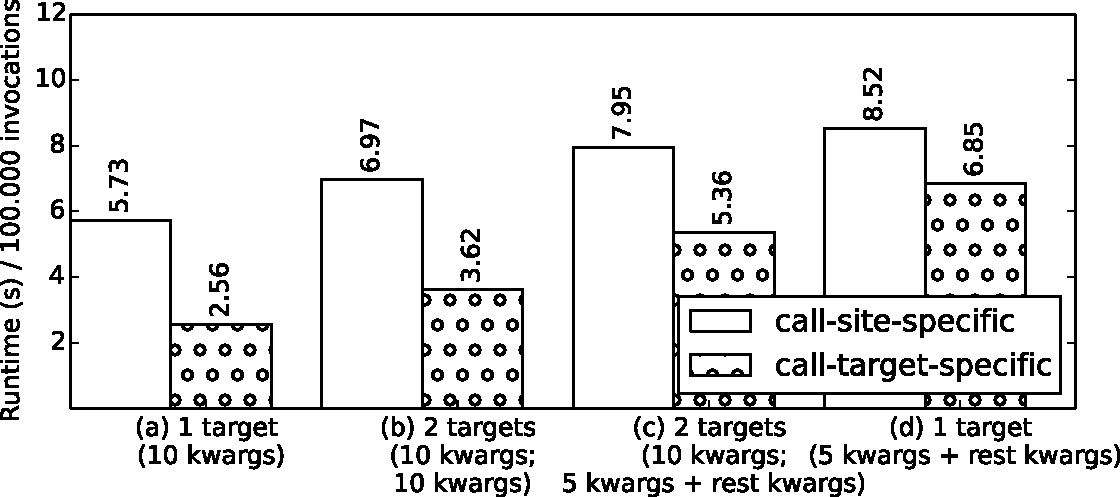
\includegraphics[width=\textwidth]{benchmark.pdf}
\end{frame}

\section{Related Work}

\end{document}
